\documentclass[12pt]{article}
\usepackage[a4paper,top=3cm,bottom=2cm,inner=3cm,outer=2cm]{geometry}
\usepackage[backend=biber,style=apa,doi=true,isbn=false,url=false]{biblatex}
\usepackage[onehalfspacing]{setspace}
\usepackage{graphicx}
\usepackage{authblk}
\usepackage{ragged2e}
\setcounter{section}{-1}
\setlength{\emergencystretch}{3em}
\addbibresource{references.bib}


\title{A Ponte entre o Design e a Engenharia de Software}
\author{Leonardo Heidi Almeida Murakami}
\affil{Instituto de Matemática e Estatística, Universidade de São Paulo}
\date{Novembro 2024}

\begin{document}

\maketitle
\section{Resumo deste Ensaio}
Este ensaio sobre o conceito de módulo tanto na Engenharia de Software e no Design busca realizar uma ponte entre os dois conceitos de modo a mostra sua similaridade - em alguns pontos - e mostrar como estas disciplinas enfrentam problemas complexos. Ambas as disciplinas se utilizam da modularidade como um principio fundamental para criar sistemas adaptáveis, escaláveis e sustentáveis, embora apliquem esse principio de maneiras distintas em seus domínios.


\noindent
As principais conclusões que foram tiradas durante o ensaio:
\begin{itemize}
    \item Fundação Conceitual Compartilhada: Ambos os campos se utilizam do principio de criar elementos "removíveis", auto-contidos e repetíveis que podem ser configurados para sistemas maiores.
    \item Gerenciamento de Complexidade: Tanto a Engenharia de Software quanto o Design usam a estrategia da modularização para quebrar sistemas complexos em componentes sustentáveis, permitindo desenvolvimento independente e modificações
    \item Balança da Flexibilidade-Padronização: Ambas as disciplinas lutam com a tensão de construir uma interface padronizada enquanto permite uma flexibilidade interna e mantém a capacidade de adaptação
    \item Otimização invés de maximização: O sucesso para os dois não vem de maximizar a modularidade, mas sim de encontrar o balanco ótimo para um contexto e requisitos especifico
\end{itemize}
\section{Introdução}

No complexo cenário do desenvolvimento de produtos o Design e a Engenharia de Software frequentemente entrelaçam suas contribuições e, mesmo assim, mantém papéis distintos e complementares que frequentemente são mal compreendidos. Em seu núcleo, ambas as disciplinas compartilham uma estratégia fundamental de resolver seus problemas através da modularidade - o princípio de criar elementos auto-contidos e reusáveis que podem ser reconfigurados em um escopo maior. Esse paralelo revela uma dinâmica fascinante: enquanto o Engenheiro de Software implementa a modularidade através de componentes de código e arquitetura de sistemas, o Design aplica a modularidade através de elementos padronizados e sistemas adaptáveis que fazem a ponte da tecnologia com as necessidades humanas

Em vez de enxergarmos um campo fagocitando o outro, nós deveriamos entender como ambas as disciplinas se utilizam da modularidade para lidar com a complexidade, balancear a padronização com a flexibilidade e para atingir soluções escaláveis. Esse ensaio irá explorar a relação entre esses campos, examinando como suas abordagens paralelas à modularidade se complementam e, ao mesmo tempo, mantêm suas identidades metodológicas distintas na criação de produtos e soluções bem-sucedidos.

\section{A Ponte modular: Paralelo entre a Engenharia de Software e o Design}

Tanto na engenharia de software e no design, o principio da modularidade molda como os praticantes aproximam problemas complexos. Enquanto esses campos parecem distintos num primeiro olhar, sua abordagem subjacente à modularidade revela semelhanças impressionantes em termos de metodologia e filosofia.

\subsection{O conceito principal da modularidade}

O conceito de modularidade em ambas as disciplinas dependem naquilo que pode ser descrito como elementos que devem ser destacáveis, autocontidos e repetíveis, permitindo sua reconfiguração e padronização em um sistema mais amplo. Similarmente, na Engenharia de Software, a programação modular enfatiza a criação de componentes de código independentes e reutilizáveis que podem ser montados em aplicações maiores.

\subsection{Gerenciamento de complexidade através da modularidade}

Esse paralelo se torna evidente quando examinamos como ambos os campos utilizam a modularidade para lidar com a complexidade. Assim como os Designers utilizam sistemas modulares para, por exemplo, criar mobilha que pode ser reconfigurada e adaptada para lidar com espaços diferentes, os Engenheiros de Software aplicam a arquitetura modular para construir aplicações que podem ser modificadas e expandidas sem interromper todo o sistema. Ambas as abordagens compartilham a característica fundamental da multiconfigurabilidade, que é a capacidade de atingir resultados variáveis a partir de uma quantidade limitada de entradas padronizadas.

\subsection{Equilíbrio entre flexibilidade e padronização}

A similaridade continua quando ambos os campos se aproximam do tópico do equilíbrio entre a flexibilidade e a padronização. No Design, módulos provém unidade na diversidade, permitindo a produção padronizada enquanto mantém sua adaptabilidade para contextos diferentes. A Engenharia de Software espelha isso através do principio do encapsulamento, onde interfaces padronizadas permitem flexibilidade interna enquanto mantém consistência externa. Essa característica permite que designers e engenheiros criem sistemas que são robustos e versáteis
\vspace{20px}

\noindent
\begin{minipage}{0.4\textwidth}

\includegraphics[width=1\textwidth]{pax-ikea.png}
\end{minipage}
\begin{minipage}{0.6\textwidth}\raggedright
O guarda-roupa PAX da IKEA tem alguns tamanhos padronizados (60 cm, 75 cm, 100 cm de largura), mas oferece infinitas possibilidades de configurações internas. Os tamanhos externas ficam inalteradas para que exista uma eficácia da produção, enquanto os componentes internos (gavetas, prateleiras, barras) podem ser organizados de diversas formas para suprir as demandas individuais.
\end{minipage}

\vspace{5px}

\noindent
\begin{minipage}{0.6\textwidth}\raggedright
Os sistemas de mapeamento objeto-relacional (ORM) fornecem interfaces padronizadas para operações de banco de dados e permitem que diferentes mecanismos de banco de dados (MySQL, PostgreSQL, MongoDB) sejam trocados por baixo dos panos sem influencia no desenvolvedor.
A API externa permanece consistente para os desenvolvedores, enquanto a implementação interna pode ser altamente personalizada para diferentes tecnologias de banco de dados.
\end{minipage}
\begin{minipage}{0.4\textwidth}
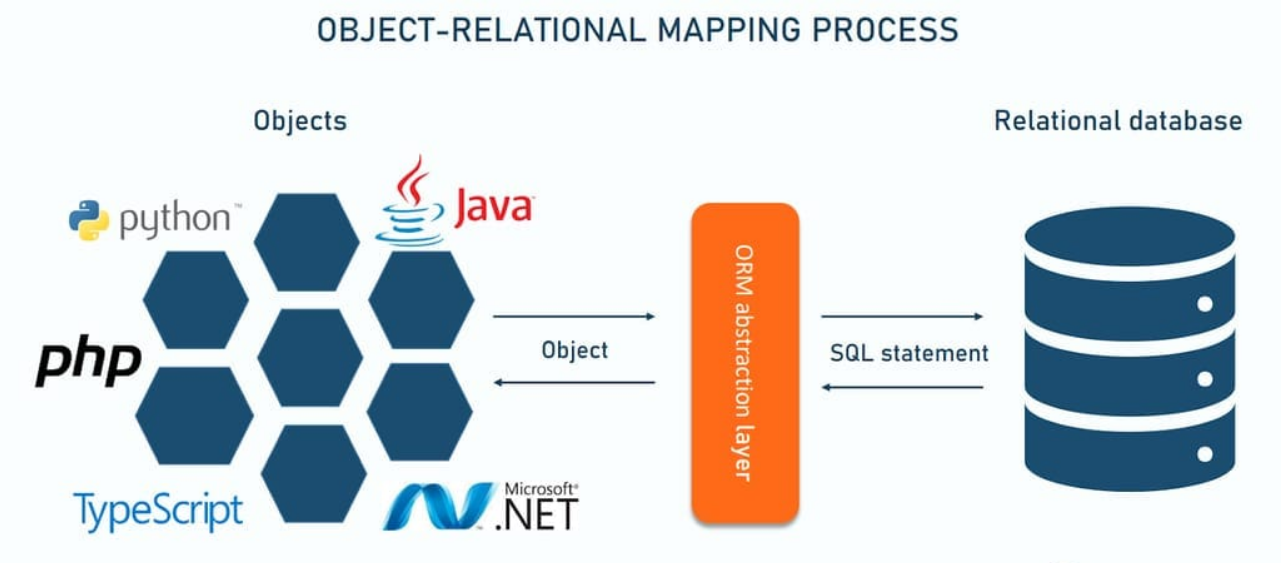
\includegraphics[width=1\textwidth]{orm.png}
\end{minipage}


\vspace{20px}
Ambos exemplos mostram como "o módulo permite que se estabeleça unidade entre diversidades, como ponte, elo ou moeda de troca, como elemento de interligação da diversidade por meio desse componente de unidade." \cite{piculoportugal2024modulo}

\subsection{Racionalização e Simplificação}
Os dois campos enxergam a modularidade como um meio de atingir a racionalização e simplificação. No desenvolvimento de software isso se manifesta como o principio da separação de interesses, um conceito fundamental explorado no trabalho de \cite{parnas1972criteria} (Sobre os critérios a serem usados na decomposição de sistemas em módulos). Parnas argumenta que a eficácia da modularidade não está no simples ato de quebrar sistemas, mas sim em como escolhemos dividi-los. Ele demonstra isso através da comparação entre dois métodos diferentes e modularizar o mesmo sistema: um baseado em etapas de processamento (semelhante a um fluxograma) e outro baseado no que ele chama de “ocultação de informações”.

Parnas também observa que os benefícios esperados da programação modular devem ser:
\begin{enumerate}
    \item Gerencial - o tempo de desenvolvimento deve ser reduzido porque grupos separados podem trabalhar em cada módulo com pouca - ou nenhuma - necessidade de comunicação
    \item Flexibilidade do produto - deve ser possível fazer alterações drásticas em um módulo sem a necessidade de alterar outros, desde que se mantenha a interface definida
    \item Compreensibilidade - deve ser possível estudar o sistema um módulo de cada vez
\end{enumerate}

Estes benefícios se aplicam notavelmente bem tanto para engenharia de software quanto para o design. Nós aplicamos a modularidade para quebrar produtos complexos em unidades que podem ser produzidas, mantidas e modificadas eficientemente, simplificando todo o processo. O processo de racionalização de ambos os campos buscam encontrar aquilo que Parnas descreve como "ocultação de informações" onde cada módulo busca encapsular (ou esconder) decisões chaves de design de outros módulos. Esse princípio ajuda a gerenciar a complexidade, permitindo que sejam feitas alterações em um módulo sem afetar os outros, desde que a interface entre os módulos permaneça estável.

\subsection{Limitações da Modularidade: Beneficios e Custos}
Enquanto a modularidade oferece vantagens poderosas nos dois campos, ela introduz tensões fundamentais que os praticantes devem navegar. Essas tensões espelham uma a outra, mostrando a natureza característica de sistemas modulares.

\subsubsection{A divisão digital-analógica}
Na engenharia de software, abstrações modulares frequentemente introduzem etapas discretas que restringem a fluidez onde a variação poderia ocorrer de maneira mais natural. Interfaces de usuário mais dinâmicas, por exemplo, podem precisar se conformar a limites rígidos impostos por outros componentes, assim como uma API deve traduzir processos contínuos do mundo real em transições discretas de estado.


Da mesma forma, no design, os sistemas modulares muitas vezes precisam digitalizar realidades analógicas - um sistema de móveis modulares cria incrementos de tamanho fixo onde as soluções personalizadas fluiriam continuamente. Essa digitalização traz clareza e restrição.

\subsubsection{O Equilibrio Amplitude-Frequencia}
Ambos os campos enfrentam um compromisso crucial entre o tamanho do módulo e a adaptabilidade. Em software, módulos maiores oferecem mais coesão interna, mas reduzem a flexibilidade combinatória. Um módulo de autenticação feito de ponta a ponta é mais consistente internamente, mas menos adaptável do que componentes menores e mais focados. 

O design enfrenta o mesmo desafio: em sistemas de sinalização, usar menos tipos padronizados de placas (módulos maiores) simplifica a produção e mantém uma forte consistência visual, mas limita a precisão com que a informação pode ser transmitida em diferentes contextos. Por outro lado, criar muitas variantes especializadas de placas (módulos menores) permite uma comunicação mais detalhada, mas aumenta a complexidade do sistema e os custos de produção. Essa tensão fundamental entre o tamanho dos módulos e a adaptabilidade do sistema molda decisões em ambas as disciplinas.

\vspace{20px}
\noindent
\begin{minipage}{0.6\textwidth}\raggedright
O ecossistema de componentes do framework de Desenvolvimento Web React ilustra bem esse paradoxo. Embora os componentes individuais sejam modulares e reutilizáveis, a gestão de compatibilidade de versões e dependências entre múltiplos componentes pode se tornar extremamente complexa, especialmente em aplicações de grande escala.
\end{minipage}
\begin{minipage}{0.4\textwidth}
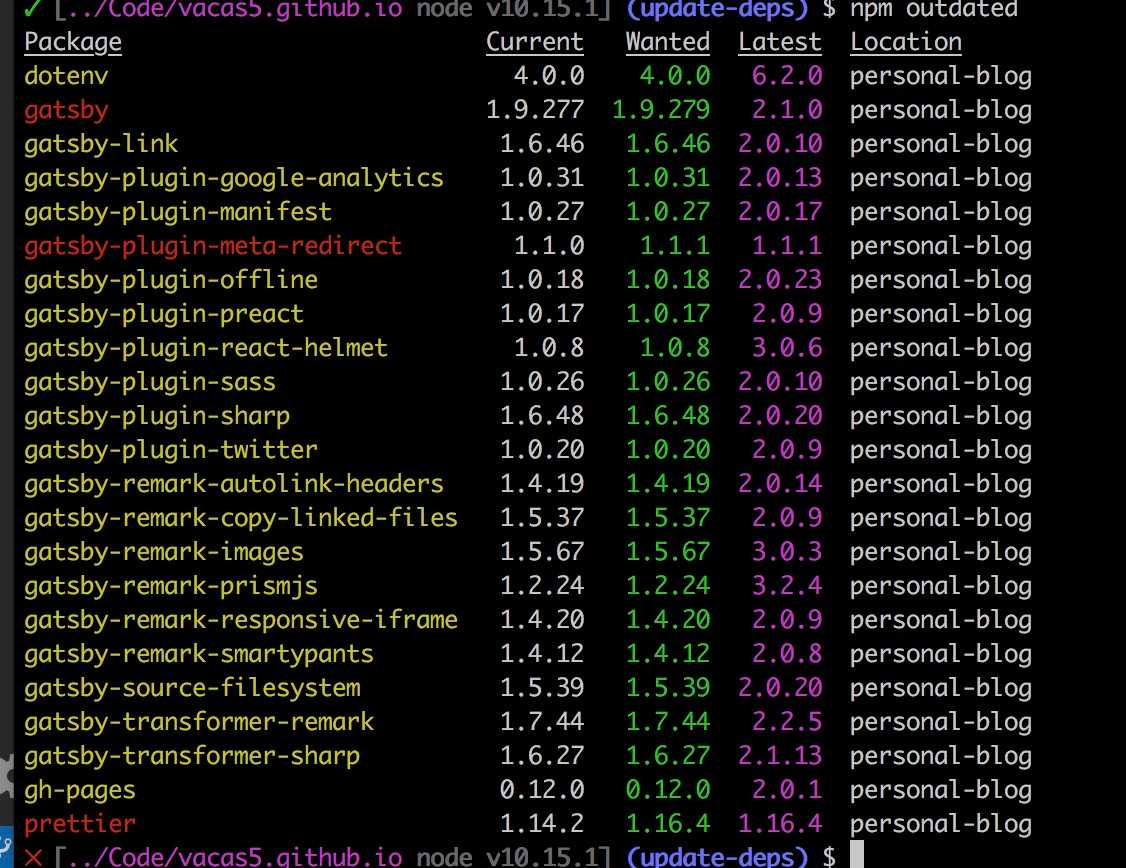
\includegraphics[width=1\textwidth]{react-deps-hell.jpg}
\end{minipage}

\vspace{5px}

\noindent
\begin{minipage}{0.4\textwidth}

\includegraphics[width=1\textwidth]{airport-signs.jpg}
\end{minipage}
\begin{minipage}{0.6\textwidth}\raggedright
De forma semelhante, em sistemas de sinalização de aeroportos, placas modulares permitem uma produção padronizada e atualizações simplificadas, mas coordenar múltiplas camadas de informação — como números de portões, pictogramas e textos multilíngues — enquanto se mantém a hierarquia visual e a compatibilidade com diferentes distâncias de visualização e condições de iluminação, adiciona uma complexidade significativa ao sistema.
\end{minipage}

\subsubsection{Achando a Harmonia}
O sucesso de sistemas modulares não reside em eliminar essas tensões, mas em encontrar o equilíbrio adequado para cada contexto. Tanto Engenheiros de Software quanto Designers devem considerar os requisitos, restrições e casos de uso específicos ao definir os limites e a granularidade dos módulos. O objetivo não é maximizar a modularidade, mas otimizá-la para as necessidades particulares de cada projeto, reconhecendo que certa tensão entre padronização e adaptação não é apenas inevitável, mas essencial para a eficácia do sistema.

\section{Bibliografia}
\renewcommand{\bibfont}{\raggedright}
\renewcommand{\bibname}{}
\renewcommand{\refname}{}
\printbibliography

\end{document}

